% Template: Fabian Wenzelmann, 2016 - 2017

\documentclass[a4paper,
  twoside, % für Unterscheidung gerade / ungerade Seite
  headlines=2.1 % Anzahl der Zeilen im Kopf, wenn man mehr verwenden will erhöhen
  ]{scrartcl}
\AddToHook{cmd/section/before}{\clearpage}

\usepackage[
  margin=2cm,
  includefoot,
  footskip=35pt,
  includeheadfoot,
  headsep=0.5cm,
]{geometry}
\usepackage[utf8]{inputenc}
\usepackage{amsmath}
\usepackage{float}
\usepackage{amssymb}
\usepackage{amsthm}
\usepackage[automark,headsepline]{scrlayer-scrpage}
\usepackage{enumerate}
\usepackage[protrusion=true,expansion=true, kerning]{microtype} % Sieht damit einfach schöner aus
\usepackage{mathtools}

% nur für das Beispiel benötigt
\usepackage{lipsum}

\newcommand{\yourname}{Ioan Oleksii Kelier} % Weitere Autor*innen mittels \and Befehl einfügen
% \newcommand{\yourname}{Dein Name \\ \texttt{123456789} \and Anderer Name \\ \texttt{987654321}} % Hier ein Bsp mit Martikelnummern, auf jeden Fall \headingname anpassen (keine newlines)
\newcommand{\headingname}{Ioan Oleksii Kelier} % Namen wie sie im Kopf erscheinen, wenn zu lang z.B. nur Nachnamen verwenden
% Auch wenn man eine Trennung durch Kommata haben will hier die Namen erneut durch Kommata getrennt wiederholen
% \newcommand{\headingname}{Dein Name, Anderer Name} % Hier ein Beispiel für eine anders formatierte Liste
\newcommand{\lecture}{Algorithms notes}
\author{\yourname}
\title{\lecture}
\date{} % Wer ein Datum auf dem Dokument haben will hier eintragen, \today erstellt das heutige Datum

\pagestyle{scrheadings}
\setkomafont{pagehead}{\normalfont}
\lohead{\lecture\\\headingname}
\lehead{\lecture\\\headingname}

%------------------------------------------------------------------------------------------------------------------------------------------------
\begin{document}

\section*{General concepts}

Algorithm is considered to be correct if:

\begin{enumerate}
    \item Algorithm calculating the correct output for each input
    \item Algorithm is terminating
\end{enumerate}

%------------------------------------------------------------------------------------------------------------------------------------------------
\section*{Sorting algorithms}

    \subsection*{Selection Sort}

    Key ideas of the algorithm: 
    \begin{itemize}
        \item Find the smallest element in array, switch it with the 1 element in array.
        \item Find the smallest element in array[2:n], switch it with the 2 element in array.
        \item \dots{}
    \end{itemize}
    Pseudo code:
    \begin{figure}[H]
        \centering
        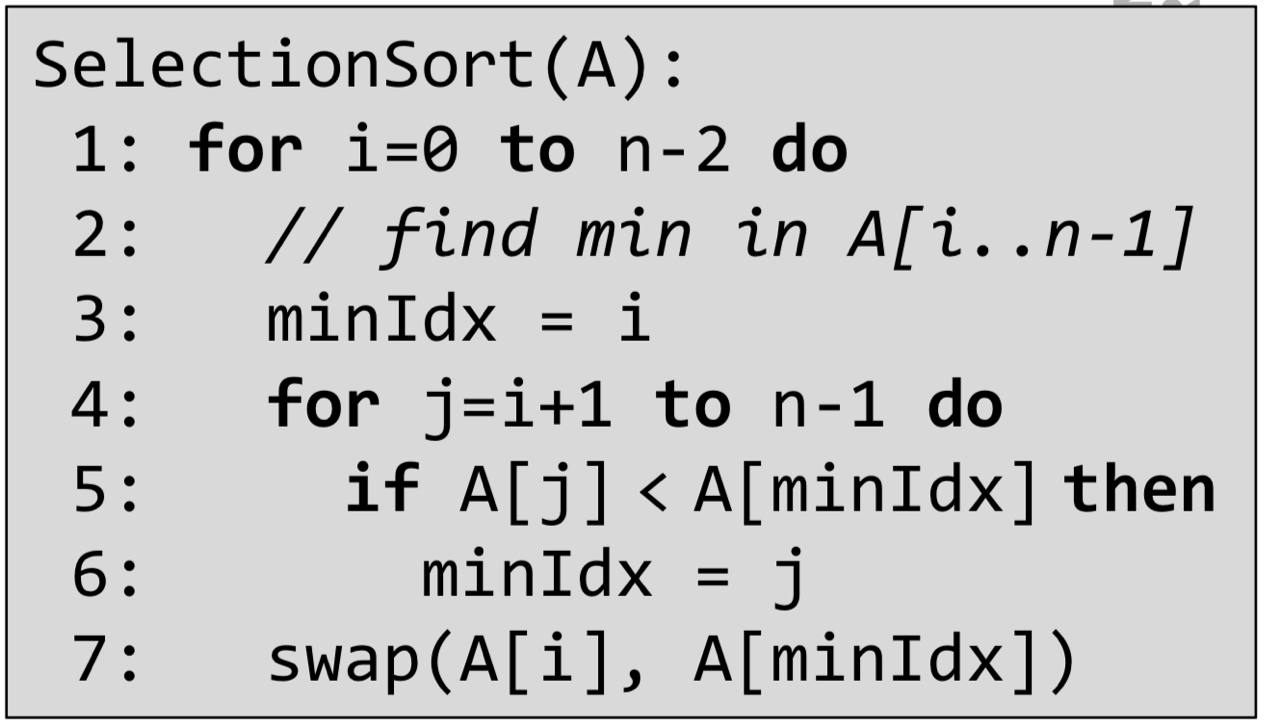
\includegraphics[width=0.3\linewidth]{image.png}
        \caption{Pseudo code for selection sort algorithm}
        \label{fig:enter-label}
    \end{figure}
    Key points from the lecture notes:
    \begin{itemize}
       \item  Main problem of the selection sort is that it becomes disproportionately slower with increasing size of the array.
       \item \textbf{Time complexity: $\mathbb{O}(n^{2})$.}
    \end{itemize}

    \clearpage
    \subsection*{Insertion sort}

    Key ideas of the algorithm:
    \begin{itemize}
        \item Gradually always add the next element to the already sorted part.
        
        \item We are swapping elements until either pos of current element is 0, which means that we reached start of our array, (for example part \textit{(d)} in Figure 2) or until we find element which is smaller then the current one (for example part \textit{(e)} in Figure 2).

        \item Efficiency depends on the following part: \textit{how nearly sorted the input array is}? It's important due to the fact that we may need to go all the way back to the last sorted element.

        \item \textbf{Time complexity: $\mathbb{O}(n^{2})$}
    \end{itemize}
    Pseudo code:
    \begin{figure}[H]
        \centering
        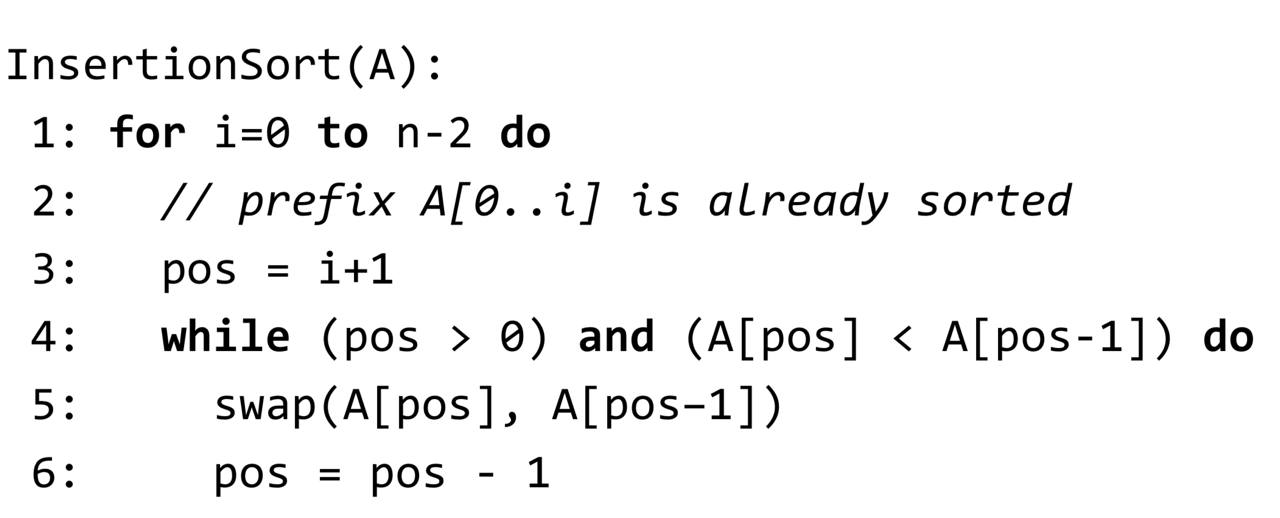
\includegraphics[width=0.5\linewidth]{insertion_sort_pseudocode.png}
        \caption{Insertion sort pseudo code}
        \label{fig:enter-label}
    \end{figure}
    Illustration of the algorithm:
    \begin{figure}[H]
        \centering
        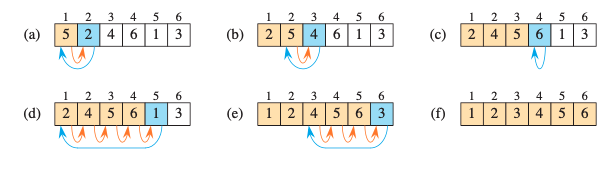
\includegraphics[width=0.7\linewidth]{insertion_sort_algo.png}
        \caption{Insertion sort algorithm}
        \label{fig:enter-label}
    \end{figure}


    












    
\end{document}